% Options for packages loaded elsewhere
\PassOptionsToPackage{unicode}{hyperref}
\PassOptionsToPackage{hyphens}{url}
%
\documentclass[
  12 pt,
  a4paper,
]{article}
\usepackage{amsmath,amssymb}
\usepackage{setspace}
\usepackage{iftex}
\ifPDFTeX
  \usepackage[T1]{fontenc}
  \usepackage[utf8]{inputenc}
  \usepackage{textcomp} % provide euro and other symbols
\else % if luatex or xetex
  \usepackage{unicode-math} % this also loads fontspec
  \defaultfontfeatures{Scale=MatchLowercase}
  \defaultfontfeatures[\rmfamily]{Ligatures=TeX,Scale=1}
\fi
\usepackage{lmodern}
\ifPDFTeX\else
  % xetex/luatex font selection
  \setmainfont[]{Times New Roman}
\fi
% Use upquote if available, for straight quotes in verbatim environments
\IfFileExists{upquote.sty}{\usepackage{upquote}}{}
\IfFileExists{microtype.sty}{% use microtype if available
  \usepackage[]{microtype}
  \UseMicrotypeSet[protrusion]{basicmath} % disable protrusion for tt fonts
}{}
\makeatletter
\@ifundefined{KOMAClassName}{% if non-KOMA class
  \IfFileExists{parskip.sty}{%
    \usepackage{parskip}
  }{% else
    \setlength{\parindent}{0pt}
    \setlength{\parskip}{6pt plus 2pt minus 1pt}}
}{% if KOMA class
  \KOMAoptions{parskip=half}}
\makeatother
\usepackage{xcolor}
\usepackage[margin=1in]{geometry}
\usepackage{color}
\usepackage{fancyvrb}
\newcommand{\VerbBar}{|}
\newcommand{\VERB}{\Verb[commandchars=\\\{\}]}
\DefineVerbatimEnvironment{Highlighting}{Verbatim}{commandchars=\\\{\}}
% Add ',fontsize=\small' for more characters per line
\usepackage{framed}
\definecolor{shadecolor}{RGB}{248,248,248}
\newenvironment{Shaded}{\begin{snugshade}}{\end{snugshade}}
\newcommand{\AlertTok}[1]{\textcolor[rgb]{0.94,0.16,0.16}{#1}}
\newcommand{\AnnotationTok}[1]{\textcolor[rgb]{0.56,0.35,0.01}{\textbf{\textit{#1}}}}
\newcommand{\AttributeTok}[1]{\textcolor[rgb]{0.13,0.29,0.53}{#1}}
\newcommand{\BaseNTok}[1]{\textcolor[rgb]{0.00,0.00,0.81}{#1}}
\newcommand{\BuiltInTok}[1]{#1}
\newcommand{\CharTok}[1]{\textcolor[rgb]{0.31,0.60,0.02}{#1}}
\newcommand{\CommentTok}[1]{\textcolor[rgb]{0.56,0.35,0.01}{\textit{#1}}}
\newcommand{\CommentVarTok}[1]{\textcolor[rgb]{0.56,0.35,0.01}{\textbf{\textit{#1}}}}
\newcommand{\ConstantTok}[1]{\textcolor[rgb]{0.56,0.35,0.01}{#1}}
\newcommand{\ControlFlowTok}[1]{\textcolor[rgb]{0.13,0.29,0.53}{\textbf{#1}}}
\newcommand{\DataTypeTok}[1]{\textcolor[rgb]{0.13,0.29,0.53}{#1}}
\newcommand{\DecValTok}[1]{\textcolor[rgb]{0.00,0.00,0.81}{#1}}
\newcommand{\DocumentationTok}[1]{\textcolor[rgb]{0.56,0.35,0.01}{\textbf{\textit{#1}}}}
\newcommand{\ErrorTok}[1]{\textcolor[rgb]{0.64,0.00,0.00}{\textbf{#1}}}
\newcommand{\ExtensionTok}[1]{#1}
\newcommand{\FloatTok}[1]{\textcolor[rgb]{0.00,0.00,0.81}{#1}}
\newcommand{\FunctionTok}[1]{\textcolor[rgb]{0.13,0.29,0.53}{\textbf{#1}}}
\newcommand{\ImportTok}[1]{#1}
\newcommand{\InformationTok}[1]{\textcolor[rgb]{0.56,0.35,0.01}{\textbf{\textit{#1}}}}
\newcommand{\KeywordTok}[1]{\textcolor[rgb]{0.13,0.29,0.53}{\textbf{#1}}}
\newcommand{\NormalTok}[1]{#1}
\newcommand{\OperatorTok}[1]{\textcolor[rgb]{0.81,0.36,0.00}{\textbf{#1}}}
\newcommand{\OtherTok}[1]{\textcolor[rgb]{0.56,0.35,0.01}{#1}}
\newcommand{\PreprocessorTok}[1]{\textcolor[rgb]{0.56,0.35,0.01}{\textit{#1}}}
\newcommand{\RegionMarkerTok}[1]{#1}
\newcommand{\SpecialCharTok}[1]{\textcolor[rgb]{0.81,0.36,0.00}{\textbf{#1}}}
\newcommand{\SpecialStringTok}[1]{\textcolor[rgb]{0.31,0.60,0.02}{#1}}
\newcommand{\StringTok}[1]{\textcolor[rgb]{0.31,0.60,0.02}{#1}}
\newcommand{\VariableTok}[1]{\textcolor[rgb]{0.00,0.00,0.00}{#1}}
\newcommand{\VerbatimStringTok}[1]{\textcolor[rgb]{0.31,0.60,0.02}{#1}}
\newcommand{\WarningTok}[1]{\textcolor[rgb]{0.56,0.35,0.01}{\textbf{\textit{#1}}}}
\usepackage{longtable,booktabs,array}
\usepackage{calc} % for calculating minipage widths
% Correct order of tables after \paragraph or \subparagraph
\usepackage{etoolbox}
\makeatletter
\patchcmd\longtable{\par}{\if@noskipsec\mbox{}\fi\par}{}{}
\makeatother
% Allow footnotes in longtable head/foot
\IfFileExists{footnotehyper.sty}{\usepackage{footnotehyper}}{\usepackage{footnote}}
\makesavenoteenv{longtable}
\usepackage{graphicx}
\makeatletter
\def\maxwidth{\ifdim\Gin@nat@width>\linewidth\linewidth\else\Gin@nat@width\fi}
\def\maxheight{\ifdim\Gin@nat@height>\textheight\textheight\else\Gin@nat@height\fi}
\makeatother
% Scale images if necessary, so that they will not overflow the page
% margins by default, and it is still possible to overwrite the defaults
% using explicit options in \includegraphics[width, height, ...]{}
\setkeys{Gin}{width=\maxwidth,height=\maxheight,keepaspectratio}
% Set default figure placement to htbp
\makeatletter
\def\fps@figure{htbp}
\makeatother
\setlength{\emergencystretch}{3em} % prevent overfull lines
\providecommand{\tightlist}{%
  \setlength{\itemsep}{0pt}\setlength{\parskip}{0pt}}
\setcounter{secnumdepth}{-\maxdimen} % remove section numbering
\ifLuaTeX
\usepackage[bidi=basic]{babel}
\else
\usepackage[bidi=default]{babel}
\fi
\babelprovide[main,import]{spanish}
\ifPDFTeX
\else
\babelfont{rm}[]{Times New Roman}
\fi
% get rid of language-specific shorthands (see #6817):
\let\LanguageShortHands\languageshorthands
\def\languageshorthands#1{}
\ifLuaTeX
  \usepackage{selnolig}  % disable illegal ligatures
\fi
\usepackage{bookmark}
\IfFileExists{xurl.sty}{\usepackage{xurl}}{} % add URL line breaks if available
\urlstyle{same}
\hypersetup{
  pdftitle={U4. Sistema d'arxius. Ubuntu},
  pdfauthor={by tofermos},
  pdflang={es-ES},
  hidelinks,
  pdfcreator={LaTeX via pandoc}}

\title{U4. Sistema d'arxius. Ubuntu}
\author{by tofermos}
\date{}

\begin{document}
\maketitle

{
\setcounter{tocdepth}{2}
\tableofcontents
}
\setstretch{1.5}
\newpage
\renewcommand\tablename{Tabla}

\begin{center}\rule{0.5\linewidth}{0.5pt}\end{center}

\section{1. Introducció}\label{introducciuxf3}

Un sistema d'arxius és una estructura que un sistema operatiu utilitza
per a organitzar i emmagatzemar dades de manera eficient en un
dispositiu d'emmagatzematge (disc dur, SSD, etc.). El sistema de fitxers
és essencial per a garantir que els arxius es puguen crear, modificar i
eliminar de manera segura i controlada.

Els sistemes operatius basats en Linux, com Lubuntu, ofereixen diversos
tipus de sistemes de fitxers, cadascun amb les seues característiques. A
més, mitjançant la línia de comandes (terminal), es poden realitzar
operacions avançades sobre els arxius i directoris de manera eficient.

\section{2. Els arxius}\label{els-arxius}

Els arxius són els elements bàsics del sistema d'emmagatzematge. En
Linux, qualsevol cosa és un fitxer, incloent dispositius, processos i
sockets.

\subsection{2.1 Els comodins}\label{els-comodins}

Els comodins són caràcters especials que permeten operar sobre múltiples
arxius de manera més eficient.

\begin{longtable}[]{@{}
  >{\raggedright\arraybackslash}p{(\columnwidth - 4\tabcolsep) * \real{0.2759}}
  >{\raggedright\arraybackslash}p{(\columnwidth - 4\tabcolsep) * \real{0.4138}}
  >{\raggedright\arraybackslash}p{(\columnwidth - 4\tabcolsep) * \real{0.3103}}@{}}
\toprule\noalign{}
\begin{minipage}[b]{\linewidth}\raggedright
Comodí
\end{minipage} & \begin{minipage}[b]{\linewidth}\raggedright
Descripció
\end{minipage} & \begin{minipage}[b]{\linewidth}\raggedright
Exemple
\end{minipage} \\
\midrule\noalign{}
\endhead
\bottomrule\noalign{}
\endlastfoot
\texttt{*} & Substitueix qualsevol nombre de caràcters &
\texttt{ls\ *.txt} (mostra tots els fitxers \texttt{.txt}) \\
\texttt{?} & Substitueix un sol caràcter & \texttt{ls\ arxiu?.txt}
(mostra \texttt{arxiu1.txt}, però no \texttt{arxiu11.txt}) \\
\texttt{{[}\ {]}} & Substitueix un conjunt de caràcters &
\texttt{ls\ arxiu{[}12{]}.txt} (mostra \texttt{arxiu1.txt} i
\texttt{arxiu2.txt}) \\
\end{longtable}

\subsubsection{Exemple 1}\label{exemple-1}

\begin{Shaded}
\begin{Highlighting}[]
\FunctionTok{ls} \PreprocessorTok{*}\NormalTok{.jpg}
\end{Highlighting}
\end{Shaded}

Aquest exemple llistarà tots els fitxers amb extensió \texttt{.jpg} del
directori actual.

\subsubsection{Exemple 2}\label{exemple-2}

\begin{Shaded}
\begin{Highlighting}[]
\FunctionTok{ls}\NormalTok{ document}\PreprocessorTok{[}\SpecialStringTok{12}\PreprocessorTok{]}\NormalTok{.txt}
\end{Highlighting}
\end{Shaded}

Aquest exemple mostrarà els arxius \texttt{document1.txt} i
\texttt{document2.txt}.

\subsection{2.2 Tipus d'arxius}\label{tipus-darxius}

Els arxius en Linux es poden classificar en diversos tipus: - Arxius
normals: arxius de text o binaris. - Directoris: contenidors que
emmagatzemen altres arxius. - Arxius de dispositiu: representen el
maquinari (discs, impressores). - Enllaços: referències a altres arxius.
- Arxius de sockets: usats per a la comunicació entre processos.

Per a identificar el tipus d'un arxiu:

\begin{Shaded}
\begin{Highlighting}[]
\FunctionTok{file}\NormalTok{ nom\_arxiu}
\end{Highlighting}
\end{Shaded}

\subsubsection{Exemple}\label{exemple}

\begin{Shaded}
\begin{Highlighting}[]
\FunctionTok{file}\NormalTok{ /bin/bash}
\end{Highlighting}
\end{Shaded}

Aquesta ordre indicarà que \texttt{/bin/bash} és un executable binari.

\section{3. Els permisos d'arxius}\label{els-permisos-darxius}

Cada arxiu o directori en Linux té associats permisos que controlen qui
pot llegir, escriure o executar l'arxiu.

\begin{longtable}[]{@{}lll@{}}
\toprule\noalign{}
Permís & Descripció & ordre \\
\midrule\noalign{}
\endhead
\bottomrule\noalign{}
\endlastfoot
\texttt{r} & Lectura & Permet llegir el contingut de l'arxiu \\
\texttt{w} & Escriptura & Permet modificar l'arxiu \\
\texttt{x} & Execució & Permet executar l'arxiu com un programa \\
\end{longtable}

Els permisos s'assignen per a tres categories: - Propietari (u) - Grup
(g) - Altres (o)

Per a veure els permisos:

\begin{Shaded}
\begin{Highlighting}[]
\FunctionTok{ls} \AttributeTok{{-}l}
\end{Highlighting}
\end{Shaded}

\subsubsection{Exemple}\label{exemple-3}

\begin{Shaded}
\begin{Highlighting}[]
\FunctionTok{ls} \AttributeTok{{-}l}\NormalTok{ document.txt}
\end{Highlighting}
\end{Shaded}

Això mostrarà els permisos del fitxer \texttt{document.txt}, per
exemple:

\begin{verbatim}
-rw-r--r-- 1 usuari grup 1234 oct 13 08:42 document.txt
\end{verbatim}

\section{4. Operacions comunes
d'arxius}\label{operacions-comunes-darxius}

\begin{longtable}[]{@{}
  >{\raggedright\arraybackslash}p{(\columnwidth - 4\tabcolsep) * \real{0.2286}}
  >{\raggedright\arraybackslash}p{(\columnwidth - 4\tabcolsep) * \real{0.4381}}
  >{\raggedright\arraybackslash}p{(\columnwidth - 4\tabcolsep) * \real{0.3333}}@{}}
\toprule\noalign{}
\begin{minipage}[b]{\linewidth}\raggedright
Operació
\end{minipage} & \begin{minipage}[b]{\linewidth}\raggedright
Descripció
\end{minipage} & \begin{minipage}[b]{\linewidth}\raggedright
ordre
\end{minipage} \\
\midrule\noalign{}
\endhead
\bottomrule\noalign{}
\endlastfoot
Llistar arxius & Mostra els arxius del directori actual & \texttt{ls} \\
Copiar arxius & Copia un arxiu a una altra ubicació &
\texttt{cp\ fitxer\_origen\ fitxer\_desti} \\
Moure o canviar nom & Mou o canvia el nom d'un arxiu &
\texttt{mv\ fitxer\_origen\ fitxer\_desti} \\
Eliminar arxius & Esborra un arxiu & \texttt{rm\ fitxer} \\
Crear un arxiu buit & Crea un arxiu buit &
\texttt{touch\ nom\_fitxer} \\
Consultar el contingut & Mostra el contingut d'un arxiu de text &
\texttt{cat\ fitxer}, \texttt{less\ fitxer} \\
\end{longtable}

\subsubsection{Exemple 1: Copiar un
fitxer}\label{exemple-1-copiar-un-fitxer}

\begin{Shaded}
\begin{Highlighting}[]
\FunctionTok{cp}\NormalTok{ document.txt /home/usuari/Documentos/}
\end{Highlighting}
\end{Shaded}

\subsubsection{Exemple 2: Eliminar un
fitxer}\label{exemple-2-eliminar-un-fitxer}

\begin{Shaded}
\begin{Highlighting}[]
\FunctionTok{rm}\NormalTok{ document.txt}
\end{Highlighting}
\end{Shaded}

\subsubsection{Exemple 3: Crear un fitxer
buit}\label{exemple-3-crear-un-fitxer-buit}

\begin{Shaded}
\begin{Highlighting}[]
\FunctionTok{touch}\NormalTok{ nou\_fitxer.txt}
\end{Highlighting}
\end{Shaded}

\section{5. Els directoris}\label{els-directoris}

Els directoris són arxius especials que contenen altres arxius i
directoris. Permeten estructurar i organitzar el sistema de fitxers de
manera jeràrquica.

\subsection{5.1 Els permisos dels
directoris}\label{els-permisos-dels-directoris}

Els permisos per a directoris funcionen de manera similar als arxius,
però amb algunes diferències: - \texttt{r} (lectura): permet llistar els
continguts del directori. - \texttt{w} (escriptura): permet crear o
eliminar fitxers dins del directori. - \texttt{x} (execució): permet
accedir a un directori (canviar-hi).

Per a canviar permisos a un directori:

\begin{Shaded}
\begin{Highlighting}[]
\FunctionTok{chmod}\NormalTok{ u+rwx nom\_directori}
\end{Highlighting}
\end{Shaded}

\subsection{5.2 Operacions comunes amb els
directoris}\label{operacions-comunes-amb-els-directoris}

\begin{longtable}[]{@{}
  >{\raggedright\arraybackslash}p{(\columnwidth - 4\tabcolsep) * \real{0.2456}}
  >{\raggedright\arraybackslash}p{(\columnwidth - 4\tabcolsep) * \real{0.4298}}
  >{\raggedright\arraybackslash}p{(\columnwidth - 4\tabcolsep) * \real{0.3246}}@{}}
\toprule\noalign{}
\begin{minipage}[b]{\linewidth}\raggedright
Operació
\end{minipage} & \begin{minipage}[b]{\linewidth}\raggedright
Descripció
\end{minipage} & \begin{minipage}[b]{\linewidth}\raggedright
ordre
\end{minipage} \\
\midrule\noalign{}
\endhead
\bottomrule\noalign{}
\endlastfoot
Crear un directori & Crea un nou directori &
\texttt{mkdir\ nom\_directori} \\
Eliminar un directori buit & Esborra un directori &
\texttt{rmdir\ nom\_directori} \\
Eliminar un directori amb contingut & Esborra un directori i tots els
seus arxius & \texttt{rm\ -r\ nom\_directori} \\
Canviar de directori & Navegar entre directoris &
\texttt{cd\ nom\_directori} \\
Llistar el contingut & Llistar el contingut d'un directori &
\texttt{ls\ nom\_directori} \\
\end{longtable}

\subsubsection{Exemple 1: Crear un
directori}\label{exemple-1-crear-un-directori}

\begin{Shaded}
\begin{Highlighting}[]
\FunctionTok{mkdir}\NormalTok{ Projecte}
\end{Highlighting}
\end{Shaded}

\subsubsection{Exemple 2: Eliminar un directori
buit}\label{exemple-2-eliminar-un-directori-buit}

\begin{Shaded}
\begin{Highlighting}[]
\FunctionTok{rmdir}\NormalTok{ Projecte}
\end{Highlighting}
\end{Shaded}

\section{6. Rutes relatives i
absolutes}\label{rutes-relatives-i-absolutes}

En Linux, una \textbf{ruta} és la forma d'accedir a un fitxer o
directori dins del sistema de fitxers. Hi ha dos tipus principals de
rutes: \textbf{relatives} i \textbf{absolutes}.

\subsection{6.1 Ruta absoluta}\label{ruta-absoluta}

Una ruta absoluta és aquella que comença des de l'arrel del sistema de
fitxers (\texttt{/}) i proporciona la ubicació completa d'un fitxer o
directori. No depèn del directori actual en què et trobes.

\subsubsection{Exemple de ruta
absoluta:}\label{exemple-de-ruta-absoluta}

\begin{Shaded}
\begin{Highlighting}[]
\ExtensionTok{/home/usuari/Documentos/document.txt}
\end{Highlighting}
\end{Shaded}

En aquest cas, la ruta comença des de l'arrel (\texttt{/}) i especifica
tot el camí fins al fitxer \texttt{document.txt}.

\subsubsection{Exemple d'ús:}\label{exemple-duxfas}

\begin{Shaded}
\begin{Highlighting}[]
\BuiltInTok{cd}\NormalTok{ /home/usuari/Documentos}
\end{Highlighting}
\end{Shaded}

Aquesta ordre et porta directament al directori \texttt{Documentos},
independentment del directori on et trobes actualment.

\subsection{6.2 Ruta relativa}\label{ruta-relativa}

Una ruta relativa es defineix respecte al directori actual. No comença
des de l'arrel, sinó des del directori en què estàs treballant. Si estàs
en un directori concret, pots utilitzar rutes relatives per accedir a
fitxers o subdirectoris dins del directori actual.

\subsubsection{Exemple de ruta
relativa:}\label{exemple-de-ruta-relativa}

Si estàs en \texttt{/home/usuari} i vols accedir a
\texttt{Documentos/document.txt}, pots utilitzar una ruta relativa:

\begin{Shaded}
\begin{Highlighting}[]
\BuiltInTok{cd}\NormalTok{ Documentos}
\end{Highlighting}
\end{Shaded}

\subsubsection{\texorpdfstring{Ús dels símbols \texttt{.} i
\texttt{..}}{Ús dels símbols . i ..}}\label{uxfas-dels-suxedmbols-.-i-..}

\begin{itemize}
\tightlist
\item
  \texttt{.} fa referència al directori actual.
\item
  \texttt{..} fa referència al directori pare (el directori
  immediatament superior).
\end{itemize}

\subsubsection{Exemple d'ús:}\label{exemple-duxfas-1}

Per a pujar un nivell en la jerarquia de directoris:

\begin{Shaded}
\begin{Highlighting}[]
\BuiltInTok{cd}\NormalTok{ ..}
\end{Highlighting}
\end{Shaded}

Per a moure's a un altre directori dins del directori pare:

\begin{Shaded}
\begin{Highlighting}[]
\BuiltInTok{cd}\NormalTok{ ../Documents}
\end{Highlighting}
\end{Shaded}

\section{7. Tipus de sistemes d'arxius}\label{tipus-de-sistemes-darxius}

Linux suporta diferents tipus de sistemes de fitxers, cadascun amb les
seues característiques.

\begin{longtable}[]{@{}
  >{\raggedright\arraybackslash}p{(\columnwidth - 2\tabcolsep) * \real{0.2571}}
  >{\raggedright\arraybackslash}p{(\columnwidth - 2\tabcolsep) * \real{0.7429}}@{}}
\toprule\noalign{}
\begin{minipage}[b]{\linewidth}\raggedright
Sistema d'arxius
\end{minipage} & \begin{minipage}[b]{\linewidth}\raggedright
Característiques
\end{minipage} \\
\midrule\noalign{}
\endhead
\bottomrule\noalign{}
\endlastfoot
ext4 & Sistema d'arxius per defecte en moltes distribucions Linux. \\
NTFS & Utilitzat per Windows, compatible amb Linux. \\
FAT32 & Compatible amb diversos sistemes operatius, limitacions de
grandària d'arxiu. \\
Btrfs & Suporta snapshots, més adequat per a sistemes avançats. \\
\end{longtable}

Per a identificar el sistema de fitxers d'una partició:

\begin{Shaded}
\begin{Highlighting}[]
\FunctionTok{df} \AttributeTok{{-}T}
\end{Highlighting}
\end{Shaded}

\subsection{7.1 El sistema de fitxers basat en
inodes}\label{el-sistema-de-fitxers-basat-en-inodes}

En Linux, el sistema de fitxers està basat en \textbf{inodes}. Un inode
és una estructura de dades que conté informació important sobre un
fitxer o directori. Cada fitxer en un sistema de fitxers de Linux té un
inode associat que actua com la seua \textbf{clau única}. L'inode no
emmagatzema el nom del fitxer ni el seu contingut, sinó que guarda
informació sobre el fitxer, com ara: - El propietari - Els permisos - La
grandària del fitxer - La data de creació i modificació - Les adreces
als blocs de dades on es troba emmagatzemat el contingut del fitxer

\subsubsection{Característiques dels
inodes}\label{caracteruxedstiques-dels-inodes}

\begin{enumerate}
\def\labelenumi{\arabic{enumi}.}
\tightlist
\item
  \textbf{Clau única}: Cada fitxer o directori té un número d'inode únic
  dins del sistema de fitxers.
\item
  \textbf{Informació associada}: Conté metadades del fitxer, com
  propietari, permisos, dates\ldots{}
\item
  \textbf{Punter als blocs de dades}: L'inode apunta als blocs del disc
  on es guarda el contingut del fitxer.
\item
  \textbf{Separació de noms i dades}: Els noms del fitxer i l'inode
  estan separats; és per això que és possible tenir múltiples noms
  (enllaços durs) apuntant al mateix inode. Diferència clau de
  Unix/Linux.
\end{enumerate}

\subsubsection{Exemple: Visualitzar el número d'inode d'un
fitxer}\label{exemple-visualitzar-el-nuxfamero-dinode-dun-fitxer}

Pots visualitzar el número d'inode associat a un fitxer (o directori)
amb l'ordre següent:

\begin{Shaded}
\begin{Highlighting}[]
\FunctionTok{ls} \AttributeTok{{-}i}\NormalTok{ nom\_fitxer}
\end{Highlighting}
\end{Shaded}

\begin{Shaded}
\begin{Highlighting}[]
\FunctionTok{stat}\NormalTok{ nom\_fitxer}
\end{Highlighting}
\end{Shaded}

\subsubsection{Inode en acció}\label{inode-en-acciuxf3}

Quan crees un fitxer en un sistema de fitxers de Linux, s'assigna un
inode per a aquest fitxer. Aquest inode manté informació sobre el
fitxer, però el nom del fitxer està associat a aquest inode dins del
directori. Quan elimines un fitxer, el sistema de fitxers només elimina
l'enllaç (link) entre el nom del fitxer i l'inode, i no allibera l'inode
fins que tots els enllaços (si hi ha més d'un) han estat eliminats.

\textbf{Resum} 1. Cada fitxer (nom) està enllaçat a un inode únic.Pot
haver més d'un (diferència amb la resta de SO) 2. L'inode conté
informació del fitxer (metadades) i apunta als blocs de dades del disc.
3. Els blocs de dades són els que emmagatzemen el contingut real del
fitxer.

\subsection{7.2 Representació
gràfica}\label{representaciuxf3-gruxe0fica}

Veiem gràficament les \textbf{etiquetes o noms de fitxers}, els
\textbf{inodes} i \textbf{l'àrea de dades} com quedarien en una còpia de
fitxer, un enllaç dur i un enllaç simbòlic.

\subsubsection{Còpia de fitxer}\label{cuxf2pia-de-fitxer}

\begin{figure}
\centering
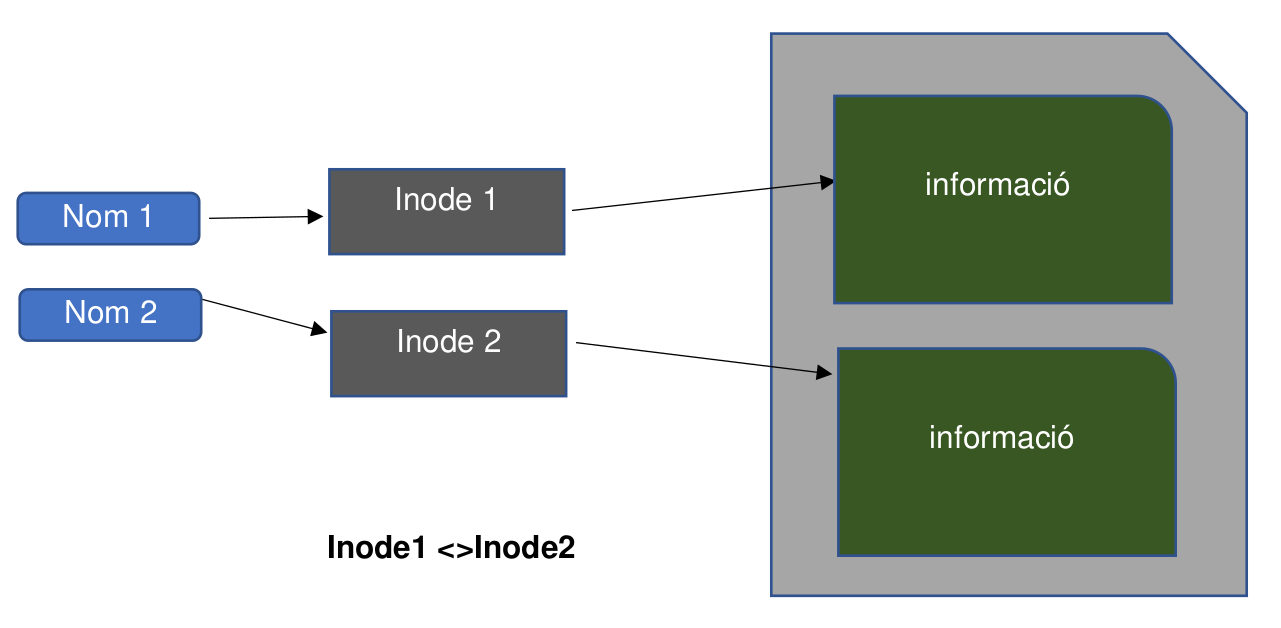
\includegraphics{png/copiadeFitxer.png}
\caption{\emph{Figura 1: Còpia de fitxer}}
\end{figure}

\subsubsection{Enllaç dur}\label{enllauxe7-dur}

\begin{figure}
\centering
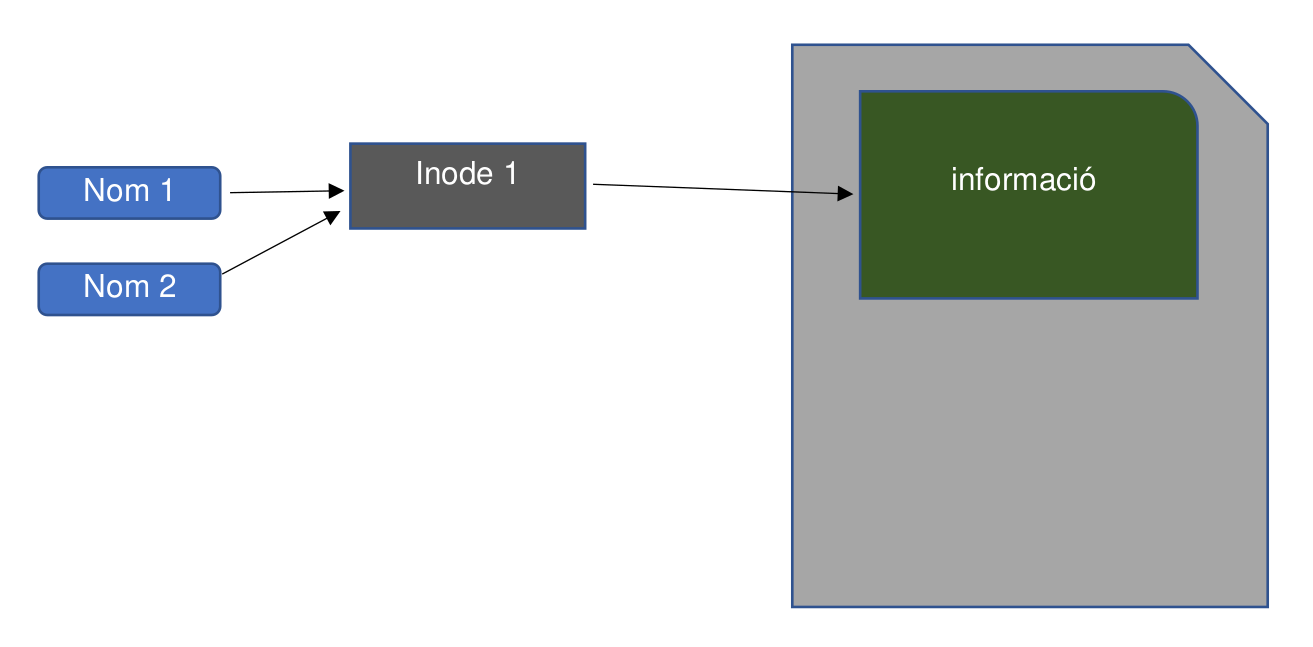
\includegraphics{png/enllaçDur.png}
\caption{\emph{Enllaç dur}}
\end{figure}

\subsubsection{Enllaç simbòlic}\label{enllauxe7-simbuxf2lic}

\begin{figure}
\centering
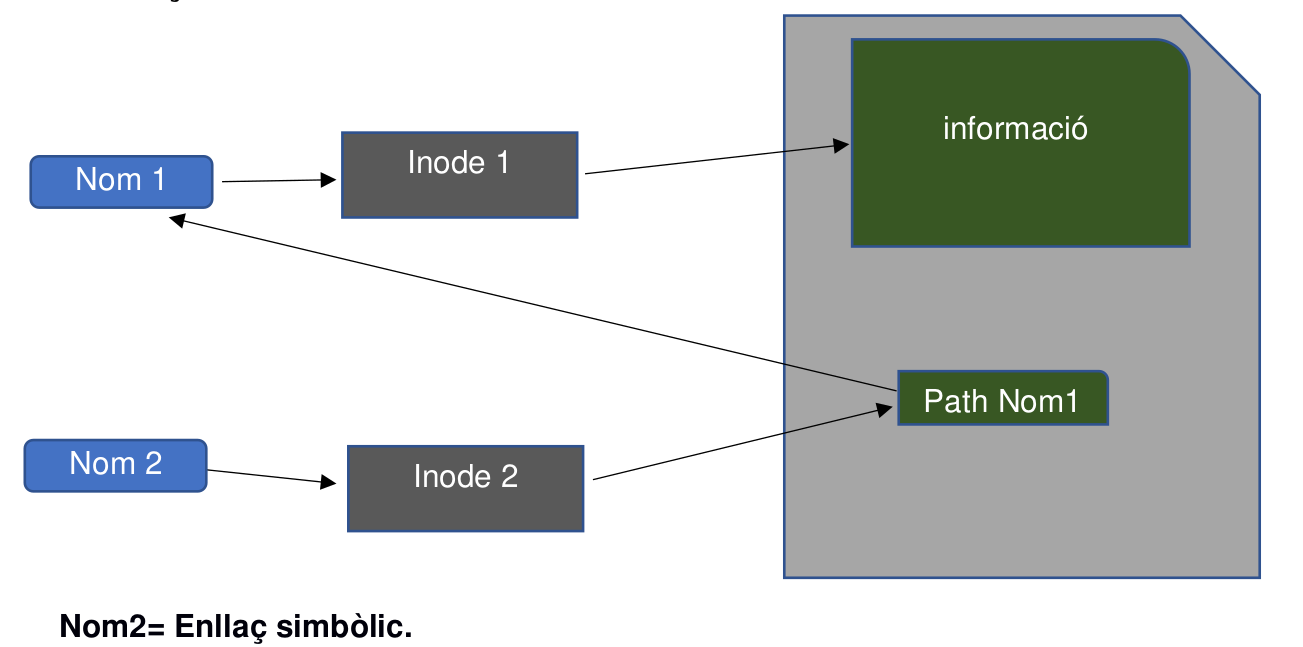
\includegraphics{png/enllaçSimbòlic.png}
\caption{\emph{Enllaç simbòlic}}
\end{figure}

\section{8. Implementació del sistema
d'arxius}\label{implementaciuxf3-del-sistema-darxius}

Un sistema de fitxers és implementat mitjançant estructures que
emmagatzemen la informació sobre els arxius i directoris, com ara taules
d'índexs (inodes) i blocs de dades.

\subsection{8.1 Comprovar el sistema
d'arxius}\label{comprovar-el-sistema-darxius}

Linux ofereix eines per a comprovar i reparar sistemes de fitxers.

\begin{Shaded}
\begin{Highlighting}[]
\ExtensionTok{fsck}\NormalTok{ /dev/sdX}
\end{Highlighting}
\end{Shaded}

Aquesta ordre comprova i repara el sistema de fitxers del dispositiu
\texttt{/dev/sdX}.

\section{9. Els sistemes
transaccionals}\label{els-sistemes-transaccionals}

Els sistemes d'arxius transaccionals permeten que les operacions
d'escriptura siguen atòmiques, garantint que qualsevol canvi es complete
amb èxit o es revertisca totalment en cas d'error. Un exemple d'això és
Btrfs, que permet utilitzar snapshots i còpies segures.

\subsection{9.1 Com utilitzar snapshots amb
Btrfs}\label{com-utilitzar-snapshots-amb-btrfs}

Un snapshot és una còpia instantània del sistema de fitxers en un moment
concret.

\begin{Shaded}
\begin{Highlighting}[]
\ExtensionTok{btrfs}\NormalTok{ subvolume snapshot /mnt/source /mnt/snapshot}
\end{Highlighting}
\end{Shaded}

Aquesta ordre crea un snapshot del volum \texttt{/mnt/source}.

\section{10. Enllaços simbòlics i enllaços
durs}\label{enllauxe7os-simbuxf2lics-i-enllauxe7os-durs}

Un enllaç simbòlic (soft link) és com un ``accés directe'' a un altre
fitxer. Un enllaç dur (hard link) fa que dos noms d'arxiu apunten al
mateix contingut.

\begin{longtable}[]{@{}
  >{\raggedright\arraybackslash}p{(\columnwidth - 2\tabcolsep) * \real{0.6129}}
  >{\raggedright\arraybackslash}p{(\columnwidth - 2\tabcolsep) * \real{0.3871}}@{}}
\toprule\noalign{}
\begin{minipage}[b]{\linewidth}\raggedright
Tipus d'enllaç
\end{minipage} & \begin{minipage}[b]{\linewidth}\raggedright
Descripció
\end{minipage} \\
\midrule\noalign{}
\endhead
\bottomrule\noalign{}
\endlastfoot
Enllaç simbòlic & Apunta a la ubicació d'un altre arxiu \\
Enllaç dur & Apunta al mateix contingut de dades dins del disc \\
\end{longtable}

\subsection{10.1 Crear un enllaç
simbòlic}\label{crear-un-enllauxe7-simbuxf2lic}

\begin{Shaded}
\begin{Highlighting}[]
\FunctionTok{ln} \AttributeTok{{-}s}\NormalTok{ fitxer\_original enllac\_simbòlic}
\end{Highlighting}
\end{Shaded}

\subsection{10.2 Crear un enllaç dur}\label{crear-un-enllauxe7-dur}

\begin{Shaded}
\begin{Highlighting}[]
\FunctionTok{ln}\NormalTok{ fitxer\_original enllac\_dur}
\end{Highlighting}
\end{Shaded}

\subsubsection{Exemple}\label{exemple-4}

\begin{Shaded}
\begin{Highlighting}[]
\FunctionTok{ln} \AttributeTok{{-}s}\NormalTok{ /home/usuari/document.txt document\_enllac.txt}
\end{Highlighting}
\end{Shaded}

\section{11. L'ordre stat}\label{lordre-stat}

L'ordre \texttt{stat} proporciona informació detallada sobre un arxiu o
directori, incloent la mida, permisos, inode i dates.

\subsubsection{Exemple d'ús}\label{exemple-duxfas-2}

\begin{Shaded}
\begin{Highlighting}[]
\FunctionTok{stat}\NormalTok{ document.txt}
\end{Highlighting}
\end{Shaded}

Aquesta ordre mostra informació completa sobre el fitxer
\texttt{document.txt}.

\section{12. L'atribut l/d/-}\label{latribut-ld-}

Quan es fa un \texttt{ls\ -l}, el primer caràcter de cada línia indica
el tipus d'arxiu: - \texttt{-} indica un arxiu normal. - \texttt{d}
indica un directori. - \texttt{l} indica un enllaç simbòlic.

\subsubsection{Exemple}\label{exemple-5}

\begin{Shaded}
\begin{Highlighting}[]
\FunctionTok{ls} \AttributeTok{{-}l}
\end{Highlighting}
\end{Shaded}

Eixida:

\begin{verbatim}
-rw-r--r-- 1 usuari grup 1234 oct 13 08:42 document.txt
drwxr-xr-x 2 usuari grup 4096 oct 13 08:42 carpeta
lrwxrwxrwx 1 usuari grup   12 oct 13 08:42 enllac -> document.txt
\end{verbatim}

En aquest exemple, \texttt{document.txt} és un arxiu normal,
\texttt{carpeta} és un directori i \texttt{enllac} és un enllaç
simbòlic.

\section{13. Empaquetament i compressió de
fitxers}\label{empaquetament-i-compressiuxf3-de-fitxers}

Empaquetar i comprimir són dues operacions relacionades però diferents.
\textbf{Empaquetar} consisteix a ajuntar diversos fitxers en un sol
arxiu, mentre que \textbf{comprimir} implica reduir la grandària d'un o
més arxius mitjançant un algoritme de compressió.

\subsection{13.1 Empaquetament amb tar}\label{empaquetament-amb-tar}

L'ordre \texttt{tar} s'utilitza per a empaquetar diversos fitxers en un
sol arxiu. El format \texttt{tar} no realitza compressió per si mateix,
simplement empaqueta fitxers i directoris en un únic arxiu.

\subsubsection{Paràmetres més comuns de l'ordre
tar}\label{paruxe0metres-muxe9s-comuns-de-lordre-tar}

\begin{longtable}[]{@{}
  >{\raggedright\arraybackslash}p{(\columnwidth - 2\tabcolsep) * \real{0.4783}}
  >{\raggedright\arraybackslash}p{(\columnwidth - 2\tabcolsep) * \real{0.5217}}@{}}
\toprule\noalign{}
\begin{minipage}[b]{\linewidth}\raggedright
Paràmetre
\end{minipage} & \begin{minipage}[b]{\linewidth}\raggedright
Descripció
\end{minipage} \\
\midrule\noalign{}
\endhead
\bottomrule\noalign{}
\endlastfoot
\texttt{-c} & Crea un arxiu empaquetat \\
\texttt{-x} & Extreu fitxers d'un arxiu empaquetat \\
\texttt{-v} & Mostra informació detallada durant l'empaquetament o
descompressió (mode detallat) \\
\texttt{-f} & Especifica el nom de l'arxiu empaquetat \\
\texttt{-z} & Comprimeix l'arxiu amb \texttt{gzip} \\
\texttt{-j} & Comprimeix l'arxiu amb \texttt{bzip2} \\
\end{longtable}

\subsubsection{Exemple d'empaquetament d'una carpeta sencera amb
tar}\label{exemple-dempaquetament-duna-carpeta-sencera-amb-tar}

\begin{Shaded}
\begin{Highlighting}[]
\FunctionTok{tar} \AttributeTok{{-}cvf}\NormalTok{ arxiu\_empaquetat.tar directori\_a\_empaquetar/}
\end{Highlighting}
\end{Shaded}

Aquest exemple empaqueta el directori complet sense comprimir-lo. El
paràmetre \texttt{-c} indica que estem creant un arxiu, \texttt{-v}
mostra els detalls i \texttt{-f} especifica el nom de l'arxiu de
destinació.

\subsubsection{Exemple d'empaquetament i compressió amb tar i
gzip}\label{exemple-dempaquetament-i-compressiuxf3-amb-tar-i-gzip}

\begin{Shaded}
\begin{Highlighting}[]
\FunctionTok{tar} \AttributeTok{{-}czvf}\NormalTok{ arxiu\_comprimit.tar.gz directori\_a\_empaquetar/}
\end{Highlighting}
\end{Shaded}

Ací s'empaqueta el directori i es comprimeix utilitzant \texttt{gzip}.
El paràmetre \texttt{-z} afegeix compressió \texttt{gzip} a l'arxiu
empaquetat.

\subsubsection{Exemple de descompressió d'un arxiu
tar.gz}\label{exemple-de-descompressiuxf3-dun-arxiu-tar.gz}

\begin{Shaded}
\begin{Highlighting}[]
\FunctionTok{tar} \AttributeTok{{-}xzvf}\NormalTok{ arxiu\_comprimit.tar.gz}
\end{Highlighting}
\end{Shaded}

Aquest exemple extreu els fitxers d'un arxiu comprimit \texttt{tar.gz}.
El paràmetre \texttt{-x} indica que s'ha d'extreure, mentre que
\texttt{-z} especifica que es tracta d'un arxiu comprimit amb
\texttt{gzip}.

\subsubsection{Exemple d'empaquetament i compressió amb tar i
bzip2}\label{exemple-dempaquetament-i-compressiuxf3-amb-tar-i-bzip2}

\begin{Shaded}
\begin{Highlighting}[]
\FunctionTok{tar} \AttributeTok{{-}cjvf}\NormalTok{ arxiu\_comprimit.tar.bz2 directori\_a\_empaquetar/}
\end{Highlighting}
\end{Shaded}

Aquest exemple utilitza \texttt{bzip2} per a comprimir l'arxiu, gràcies
al paràmetre \texttt{-j}.

\subsubsection{Exemple de descompressió d'un arxiu
tar.bz2}\label{exemple-de-descompressiuxf3-dun-arxiu-tar.bz2}

\begin{Shaded}
\begin{Highlighting}[]
\FunctionTok{tar} \AttributeTok{{-}xjvf}\NormalTok{ arxiu\_comprimit.tar.bz2}
\end{Highlighting}
\end{Shaded}

Aquesta ordre extreu un arxiu empaquetat i comprimit amb \texttt{bzip2}.

\subsection{13.2 Compressió i descompressió amb
zip}\label{compressiuxf3-i-descompressiuxf3-amb-zip}

El format \texttt{zip} és àmpliament utilitzat, especialment en sistemes
Windows, però és compatible també amb Linux. A diferència de
\texttt{tar}, \texttt{zip} empaqueta i comprimeix fitxers en un únic
pas.

\subsubsection{Exemple de compressió d'una carpeta sencera amb
zip}\label{exemple-de-compressiuxf3-duna-carpeta-sencera-amb-zip}

\begin{Shaded}
\begin{Highlighting}[]
\FunctionTok{zip} \AttributeTok{{-}r}\NormalTok{ arxiu\_comprimit.zip directori\_a\_comprimir/}
\end{Highlighting}
\end{Shaded}

En aquest exemple, el paràmetre \texttt{-r} permet comprimir tot el
directori i els seus subdirectoris de manera recursiva en un únic arxiu
\texttt{zip}.

\subsubsection{Exemple de descompressió d'un arxiu
zip}\label{exemple-de-descompressiuxf3-dun-arxiu-zip}

\begin{Shaded}
\begin{Highlighting}[]
\FunctionTok{unzip}\NormalTok{ arxiu\_comprimit.zip}
\end{Highlighting}
\end{Shaded}

Aquesta ordre descomprimeix el contingut de l'arxiu \texttt{zip} al
directori actual.

\subsection{13.3 Compressió i descompressió amb
rar}\label{compressiuxf3-i-descompressiuxf3-amb-rar}

El format \texttt{rar} és molt utilitzat en Windows i pot comprimir de
manera molt eficient. A Linux, cal instal·lar l'eina \texttt{rar} per a
poder treballar amb aquest format.

\subsubsection{Paràmetres comuns de l'ordre
rar}\label{paruxe0metres-comuns-de-lordre-rar}

\begin{longtable}[]{@{}ll@{}}
\toprule\noalign{}
Paràmetre & Descripció \\
\midrule\noalign{}
\endhead
\bottomrule\noalign{}
\endlastfoot
\texttt{a} & Afegir fitxers a un arxiu rar (comprimeix fitxers) \\
\texttt{x} & Extreu fitxers d'un arxiu rar \\
\texttt{r} & Comprimir recursivament (inclosos subdirectoris) \\
\end{longtable}

\subsubsection{Exemple de compressió d'una carpeta sencera amb
rar}\label{exemple-de-compressiuxf3-duna-carpeta-sencera-amb-rar}

\begin{Shaded}
\begin{Highlighting}[]
\ExtensionTok{rar}\NormalTok{ a }\AttributeTok{{-}r}\NormalTok{ arxiu\_comprimit.rar directori\_a\_comprimir/}
\end{Highlighting}
\end{Shaded}

El paràmetre \texttt{a} crea un arxiu comprimit. El paràmetre
\texttt{-r} assegura que es comprimeix tot el directori de manera
recursiva, incloent subdirectoris.

\subsubsection{Exemple de
descompressió}\label{exemple-de-descompressiuxf3}

D'un arxiu rar

\begin{Shaded}
\begin{Highlighting}[]
\ExtensionTok{unrar}\NormalTok{ x arxiu\_comprimit.rar}
\end{Highlighting}
\end{Shaded}

Aquesta ordre extreu tot el contingut de l'arxiu \texttt{rar}.

\subsubsection{Diferència entre empaquetar i
comprimir}\label{diferuxe8ncia-entre-empaquetar-i-comprimir}

\begin{itemize}
\tightlist
\item
  \textbf{Empaquetar}: consisteix a ajuntar diversos fitxers en un únic
  arxiu. L'arxiu resultant no es comprimeix. Exemples: arxius
  \texttt{.tar}.
\item
  \textbf{Comprimir}: es redueix la grandària de l'arxiu mitjançant
  algoritmes de compressió. Exemples: arxius \texttt{.zip},
  \texttt{.rar}, \texttt{.tar.gz}.
\end{itemize}

\subsubsection{Relació del format tar amb paquets
d'instal·lació}\label{relaciuxf3-del-format-tar-amb-paquets-dinstallaciuxf3}

El format \texttt{tar} es fa servir habitualment per a empaquetar
programari i biblioteques per a la seua distribució en sistemes Linux.
Els paquets \texttt{.tar.gz} o \texttt{.tar.bz2} encapsulen fitxers de
codi font o binaris, la qual cosa permet distribuir programari o fonts
per a la compilació i instal·lació en diverses màquines.

\subsubsection{Compatibilitat amb
Windows}\label{compatibilitat-amb-windows}

Els formats \texttt{zip} i \texttt{rar} són àmpliament utilitzats en
Windows, i són compatibles tant amb aquest sistema com amb Linux. El
format \texttt{tar} és nadiu en Linux, però pot ser utilitzat en Windows
mitjançant programari de tercers com \textbf{7-Zip} o \textbf{WinRAR},
que poden descomprimir arxius \texttt{.tar.gz} o \texttt{.tar.bz2}. Això
fa que els arxius empaquetats en Linux puguen ser utilitzats també en
Windows.

\section{13 Glossari}\label{glossari}

Clàr! A continuació et presento un glossari basat en el text que hem
tractat fins ara, amb les definicions claus per ajudar a entendre millor
els conceptes discutits.

\subsubsection{Glossari}\label{glossari-1}

\textbf{Arxiu o fitxer}: Element bàsic de magatzematge en un sistema
operatiu, que pot ser de text, binari, dispositiu, enllaç, o socket.

\textbf{Blocs de dades}: Unitats on es guarda físicament el contingut
dels arxius en un disc dins del sistema de fitxers.

\textbf{Btrfs}: Sistema d'arxius per a Linux que suporta
característiques com snapshots i còpies de seguretat.

\textbf{Carpetes}: Contenidors d'arxius que permeten organitzar el
sistema de fitxers de manera jeràrquica.

\textbf{Comodins}: Caràcters utilitzats per substituir altres caràcters
en operacions que involucren noms d'arxius.

\textbf{Directoris}: Vegeu Carpetes

\textbf{Enllaços}: Referències a arxius que poden ser simbòlics (soft
links) o durs (hard links).

\textbf{Ext4}: Sistema d'arxius estàndard per a moltes distribucions de
Linux, conegut per la seva robustesa i eficiència.

\textbf{FAT32}: Sistema d'arxius que ofereix compatibilitat amb diversos
sistemes operatius però amb limitacions en la grandària i
característiques.

\textbf{Fitxers}: Vegeu Arxiu.

\textbf{Inode}: Estructura de dades que conté informació essencial sobre
arxius i directoris, com permisos, propietari, i ubicació dels blocs de
dades.

\textbf{Linux}: Sistema operatiu de tipus Unix que és de codi obert i
utilitzat àmpliament en servidors i sistemes embebuts.

\textbf{NTFS}: Sistema d'arxius utilitzat per Windows, compatible amb
Linux a través de eines específiques.

\textbf{Permisos}: Atributs assignats a arxius i directoris que
determinen qui pot llegir, escriure, o executar-los.

\textbf{Ruta absoluta}: Camí complet des de l'arrel (/) del sistema de
fitxers fins a un arxiu o directori específic.

\textbf{Ruta relativa}: Camí que comença des del directori actual fins a
un altre arxiu o directori, no comença des de l'arrel.

\textbf{Sistema de fitxers}: Estructura organitzativa usada per un
sistema operatiu per controlar com es guarda i recupera la informació
del disc.

\textbf{Snapshots}: Funció suportada per alguns sistemes de fitxers (com
Btrfs) que permet crear una còpia instantània del sistema de fitxers en
un moment concret.

\textbf{Tar}: Utilitat que permet empaquetar múltiples arxius en un sol
arxiu, sovint usat juntament amb eines de compressió com gzip o bzip2.

\textbf{Zip/Rar}: Formats de compressió de fitxers que permeten reduir
la grandària dels fitxers emmagatzemats i suporten la compressió d'una
carpeta sencera.

\end{document}
